%-----------------------------------------------------------------------------%
\chapter{LANDASAN TEORI}
%-----------------------------------------------------------------------------%

%
\vspace{4.5pt}

\begin{flushleft}
    \begin{justify}
        \section{Tinjauan Pustaka}
    Banyak penelitian sebelumnya yang berkaitan dengan pengembangan, perancangan, dan pembuatan sebuah aplikasi menggunakan
    \textit{Systems Development Life Cycle} (SDLC) \textit{Rapid Application Development} (RAD). Dalam penelitian yang dikerjakan oleh
    Meidyan Permata Putri dan Hendra Effendi \cite{web waterfall} dihasilkan kesimpulan bahwa penerapan metode 
    RAD sudah dapat memberikan hasil maksimal ditunjukkan dengan terpenuhinya kebutuhan pengguna. Dalam penelitian yang dikerjakan oleh Abdul Rahman \cite{jurnal RAD UAT} dihasilkan kesimpulan bahwa 
    aplikasi yang telah dibuat menggunakan RAD menunjukkan penerimaan yang baik dari pengguna ditunjukkan dengan persentase pengujian \emph{User Acceptance Testing} (UAT) sebesar 91\%.
    Dalam penelitian yang dikerjakan oleh Diah Aryani, Malabay, dan Hani Dewi Ariessanti \cite{jurnal RAD UAT 2} dihasilkan kesimpulan bahwa penggunaan RAD dapat memudahkan pihak terkait dalam melakukan penelusuran dan pengelolaan umpan balik dari kuesioner dan
    pengujian UAT menghasilkan 2 nilai yaitu 91\% dari pihak kemahasiswaan dan 88\% dari pihak mahasiswa yang kedua nilai tersebut menunjukkan penerimaan pengembangan sistem dibuat.

    \vspace{1cm}
    \section{Dasar Teori}

        \subsection{\textit{Monitoring} dan Kontrol}
        Sebuah program yang dijalankan secara berkelanjutan memerlukan pemantauan 
        yang lebih detail terhadap proses pengumpulan data dan analisis informasi. 
        Pemantauan ini bertujuan untuk menyempurnakan program sehingga dapat meminimalisir 
        kesalahan. Dalam referensi \cite{Monitoring} proses pemantauan ini disebut monitoring. 
        Upaya untuk memonitor program agar berjalan sesuai tujuan maka diperlukannya suatu 
        tindakan pengendalian. Dalam referensi \cite{Kontrol} sistem ini disebut sistem kontrol. 
        \\
        \subsection{Aplikasi \textit{Mobile}}
        Program perangkat lunak yang dirancang untuk dijalankan di \emph{smartphone}, tablet, dan perangkat 
        lain disebut aplikasi \emph{mobile} \cite{mobile}. Urgensi penggunaan Aplikasi yang dikembangkan 
        berbasis mobile adalah semakin meningkatnya pengguna smartphone yang membutuhkan berbagai macam 
        alat sebagai fasilitator dalam kegiatan sehari-hari. Sebagai fasilitator, aplikasi mobile harus mampu menyediakan informasi agar dapat menjadi sumber data bagi penggunanya dan mampu meningkatkan produktifitas pengguna. 
        \\
        \subsection{\textit{Rapid Application Development} (RAD)}
        Dalam referensi \cite{Sukamto} terdapat lima tahapan yang terdapat pada model RAD, yaitu sebagai berikut:
        
        \begin{figure}[ht]
            \centering
           
	    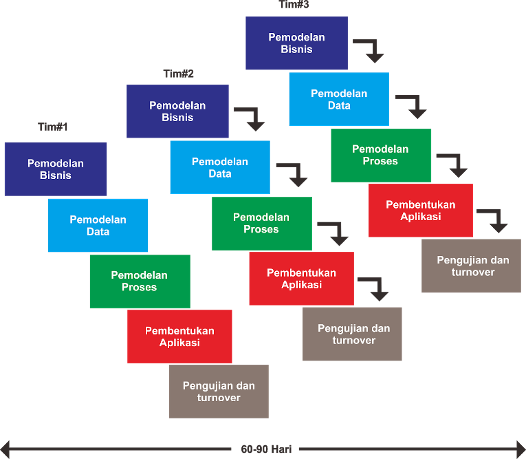
\includegraphics[width=12cm]{images/RAD.png}\\
            \caption{Gambar Ilustrasi Model RAD}
        \end{figure}
        Berdasarkan Gambar 2.1, dapat diperhatikan penjabaran sebagai berikut :
        \begin{enumerate}[label=\alph*.]
            \item Pemodelan Bisnis\\
            Pemodelan bisnis adalah serangkaian informasi mengenai produk yang dirancang. 
            dalam penelitian ini, informasi tersebut dicantumkan dalam dokumen \emph{Software Requirements Spesification} (SRS) agar dapat divalidasi oleh \emph{stakeholder}. 
            \item Pemodelan Data\\
            Pemodelan data adalah kegiatan merancang dan menghubungkan sekumpulan data berdasarkan pemodelan bisnis.
            \item Pemodelan Proses\\
            Pemodelan proses adalah kegiatan mengkonversi pemodelan data menjadi serangkaian alur proses yang bertujuan untuk menggambarkan fungsi bisnis.  
            \item Pembuatan Aplikasi\\
            Pembuatan aplikasi adalah  implementasi fungsi bisnis dan model data  kedalam bahasa pemrograman. \emph{Output} yang dihasilkan dari pembuatan aplikasi ini adalah sebuah prototipe. 
            \item Pengujian dan Pergantian\\
            Pengujian dan pergantian adalah kegiatan uji fitur yang tersedia dalam prototipe untuk mengetahui kesesuaian prototipe dengan standar yang diharapkan.\\
        \end{enumerate}

        \subsection{Flutter}
        Dalam referensi \cite{flutter} flutter merupakan framework yang menggunaan bahasa pemrograman dart yang 
        bersifat \emph{open source} (terbuka) dari Google. Flutter dapat digunakan dalam pengembangan aplikasi \emph{cross-platform} untuk penggunaan pada sistem operasi Android maupun iOS, 
        bahkan juga dapat digunakan dalam pengembangan Web ataupun Desktop dari codebase tunggal. 
        Beberapa kelebihan dari flutter adalah sudah terkoneksinya \textit{Package modules} menjadikan developer tidak harus melakukan proses manual melalui terminal, 
        sudah menggunakan konsep \textit{Object Orinented Programming} (OOP), sistem penggunaan \emph{library} yang mudah dengan hanya melakukan perubahan pada file puspec.yaml, cepatnya performa dan ketersediaan \emph{hot reload} yang sangat menyingkat waktu 
        dalam proses \emph{debug}, adanya \emph{state management} sangat memudahkan penggunaannya, dan support oleh IDE yang sering digunakan dikalangan developer seperti Android Studio dan Visual Studio Code.\\


        \subsection{\textit{Application Programming Interface} (API)}
            \textit{Application Programming Interface} (API) dapat digunakan untuk membuka akses data dan fungsionalitas dari sebuah aplikasi di perusahaan tertentu kepada pihak lain atau pihak internal di dalam perusahaan tersebut. 
            Hal ini memungkinkan terhubungnya komunikasi antar produk satu dengan lainnya serta memanfaatkan data dan fungsionalitas melalui \textit{interface} yang terdokumentasi. 
            \textit{Developer} biasa menggunakan \textit{interface} untuk menghubungkan sebuah produk dengan layanan produk lain bahkan tanpa perlu mengetahui bagaimana API diimplementasikan. 
            Penggunaan API telah menjadi hal tak terlepaskan dari pengembangan \emph{software}, sampai banyak aplikasi web paling populer saat ini tidak akan mungkin tanpa API \cite{API}. 
            API secara tradisional merujuk ke \textit{interface} yang terhubung ke aplikasi lain. Dalam aplikasi lain tersebut mungkin telah dibuat dengan salah satu bahasa pemrograman tingkat rendah, seperti Javascript. 
            API biasanya dibuat untuk HTTP serta mematuhi prinsip REST dan format JSON, menghasilkan \textit{interface} yang ramah kepada \textit{developer} dan mudah diakses serta dipahami oleh pengembangan \emph{software} 
            dan aplikasi yang dibuat dengan bahasa pemrograman yang ada saat ini.
            \\


        \subsection{\textit{Database}}
            \textit{Collection} data atau informasi yang terstruktur dan terorganisir, 
            tersimpan dalam sistem komputer dikenal sebagai \emph{database} \cite{Database}. 
            Pengelolaan \textit{database} dilakukan menggunakan \textit{Database Management System} (DBMS). 
            Data, DBMS dan aplikasi yang saling terhubung disebut sebagai sistem basis data dan familiar dengan 
            sebutan basis data. \textit{Database} yang paling umum beroperasi saat ini dimodelkan dengan 
            baris dan kolom dalam serangkaian tabel digunakan untuk meningkatkan efisiensi dalam pemanfaatan 
            kueri data. Kemudian data dengan mudah diakses untuk melakukan pengelolaan, modifikasi, 
            dan perbaharuan. Secara umum \textit{database} tidak lepas dari penggunaan \textit{structured query language} (SQL) untuk menulis 
            dan mengolah data. Salah satu SQL yang sering digunakan adalah MySQL yang merupakan perangkat lunak \textit{open source}.
            \\
        \subsection{\textit{Flowchart}}
            \textit{Flowchart} sering juga disebut dengan \textit{process flowchart, process flow diagram} atau diagram alir. Flowchart merupakan gambaran terpisah dari langkah-langkah yang tersedia dalam 
            suatu proses yang berurutan. \textit{Flowchart} sangat umum digunakan untuk berbagai tujuan,
            dapat juga berupa penggambaran sebuah proses seperti proses administrasi/layanan, proses manufaktur, atau gambaran rencana proyek \cite{Flowchart}.
            Beberapa kondisi yang disarankan untuk menggunakan \textit{flowchart} yaitu:
            \begin{enumerate}
                \item Untuk membangun pemahaman tentang bagaimana suatu proses dilakukan,
                \item Untuk mempelajari proses guna melakukan perbaikan,
                \item Untuk mengomunikasikan kepada orang lain bagaimana suatu proses dilakukan,
                \item Ketika komunikasi yang lebih baik diperlukan antara orang-orang yang terlibat dengan proses yang sama,
                \item Untuk mendokumentasikan sebuah proses saat perencanaan proyek.
            \end{enumerate} 
            \noindent \textit{Flowchart} memiliki simbol-simbol dengan arti tertentu, berdasarkan referensi \cite{gambar fc}, dapat dilihat simbol-simbol \emph{flowchart} pada gambar di bawah ini.
     
            \begin{figure}[ht]
                \centering
                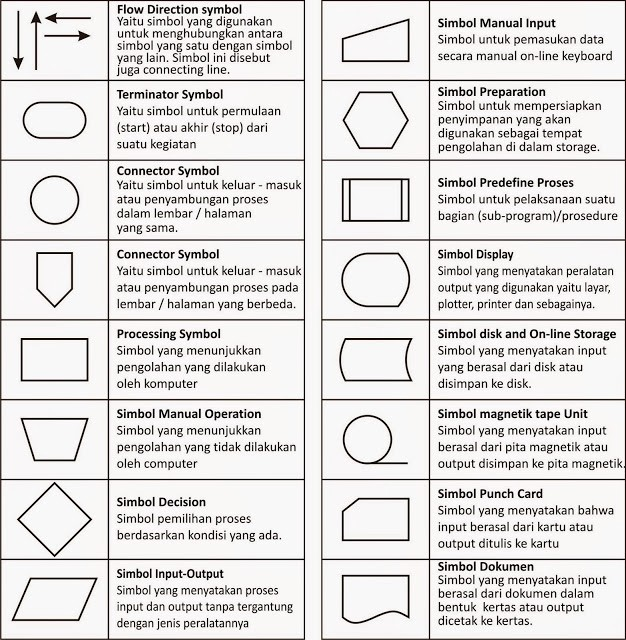
\includegraphics[width=12cm]{images/bab 2/symbol-fc.jpeg}\\
                \caption{Simbol - simbol \textit{flowchart}}
            \end{figure}
            \noindent Pada Gambar 2.2 tercantum bentuk simbol, nama, dan keterangan penggunaan simbol tersebut.\\

           
         

        \subsection{\textit{Use Case} Diagram}
            \textit{Use case} diagram adalah penggambaran yang dibuat untuk menunjukkan interaksi aktor atau pengguna dengan sistem yang dirancang, bertujuan untuk memudahkan orang lain dalam membaca informasi tersebut \cite{use case 1,use case 2}.
            Berdasarkan referensi \cite{use case 1} terdapat dua fungsi utama dari \textit{use case} dalam sebuah sistem yang dibuat, yaitu untuk memperlihatkan urutan aktivitas proses dan untuk menggambarkan \textit{bussines process}. 
            \begin{figure}[ht]
                \centering
                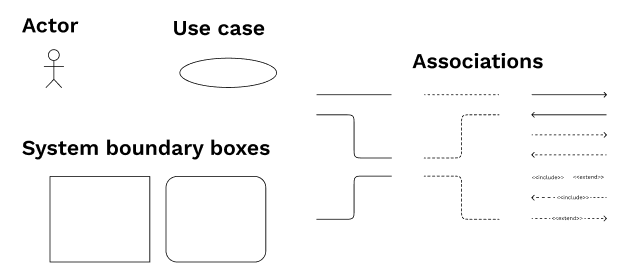
\includegraphics[width=12cm]{images/bab 2/use componen.png}
                \caption{Komponen \textit{Use case}}
            \end{figure}
            \vspace{5cm}
            \\Berdasarkan Gambar 2.3 ada beberapa komponen \emph{use case} \cite{use case 1, figma uc} yaitu, aktor, \emph{use case}, sistem, dan relasi.
            \begin{enumerate}
                \item Aktor merupakan pengguna komponen sistem untuk melakukan sesuatu dan berasal dari luar sistem. Aktor dapat berupa perangkat, manusia, atau sistem lain yang berperan.
                \item \emph{Use case} merupakan gambaran fungsional dari sebuah sistem. 
                \item Sistem merupakan komponen yang menyatakan batasan dari sistem dan memiliki relasi dengan aktor sebagai penggunanya. 
                \item \emph{Association} merupakan teknik yang digunakan menunjukkan interaksi antara komponen aktor dan \emph{use case} tetentu dan digambarkan dengan garis penghubung.\\
            \end{enumerate}
            
        \subsection{\emph{Sequence Diagram}}
        \emph{Sequence diagram} menggambarkan hubungan dan komunikasi antar objek \cite{buku scholar} sekaligus 
        menunjukkan serangkaian pesan yang diperlukan oleh objek-objek yang aktif. Objek dibaca dan diurutkan dari kiri ke kanan, 
        aktor yang menginisiasi interaksi ditaruh pada bagian paling kiri dan diikuti oleh objek setelahnya. 
        Dimensi vertikal merepresentasikan berjalannya waktu. Bagian paling atas menjadi titik awal dan 
        waktu berjalan ke bawah. Garis vertikal itu disebut juga sebagai \emph{lifeline}, pasti dimiliki setiap objek atau aktor. 
        \emph{Lifeline} ditampilkan dalam bentuk kotak yang juga dikenal sebagai \emph{activation box}. 
        ketika objek melakukan sebuah operasi, keadaan ini disebut sebagai \emph{live activation}. 
        Pesan antar objek digambarkan dengan sebuah panah yang di atasnya diberikan label keterangan.\\

        \subsection{\textit{Black Box Testing}}
        Pengujian \emph{black box} adalah salah satu metode pengujian \emph{software} yang berfokus pada bagian fungsionalitas, terkait \emph{input} dan \emph{output} yang ada apakah sudah sesuai dengan yang dituju atau belum. Tahan pengujian atau \emph{testing} merupakan hal wajib dalam siklus pengembangan perangkat lunak \cite{black box}.\\
       
       
        \subsection{\textit{User Acceptance Testing} (UAT)}
        User Acceptance Testing (UAT) adalah pengujian langsung oleh user pada pengujian akhir, dan saat berlangsungnya pengujian dilakukan pembuatan dokumen guna sebagai bukti penerimaan sistem \cite{uat} serta sebagai pengujian perangkat lunak oleh pengguna atau klien untuk menentukan apakah perangkat lunak tersebut dapat diterima atau tidak.
        \\

        \subsection{Skala \textit{Likert}}
        Skala \emph{Likert} adalah skala yang digunakan untuk mengukur sikap, pendapat, dan persepsi seseorang atau 
        sekelompok orang tentang sesuatu yang diamati. Semua pilihan jawaban diberi skor, maka responden harus 
        menggambarkan, mendukung pernyataan (positif) atau tidak mendukung pernyataan (negatif) \cite{likert}.





    \end{justify}
    



\end{flushleft}



\newpage